\documentclass[acmtog]{acmart}
\settopmatter{printacmref=false} % Removes citation information below abstract
\renewcommand\footnotetextcopyrightpermission[1]{} % removes footnote with conference information in first column
\pagestyle{plain} % removes running headers
\usepackage{graphicx}
\graphicspath{ {./fig/} }

\usepackage{booktabs} % For formal tables

% Use the "authoryear" citation style, and make sure citations are in [square brackets].
\citestyle{acmauthoryear}
\setcitestyle{square}

% A useful command for controlling the number of authors per row.
% The default value of "authorsperrow" is 2.
\settopmatter{authorsperrow=4}

% end of preamble.

\begin{document}

% Title. 
\title{Crowd Simulation: Boids++}
\subtitle{Boids Framework --- A Modern take on Craig Reynolds' Boids.}

% Authors.
\author{Di Zhao}
  \affiliation{%
    \institution{University of Califonia, Davis}}
  \email{devzhao@ucdavis.edu}

\author{Muhammad Osama}
  \affiliation{%
    \institution{University of Califonia, Davis}}
  \email{mosama@ucdavis.edu}

% abstract
\begin{abstract}
\input{tex/abstract}
\label{sec:abstract}
\end{abstract}

%keywords
\keywords{Crowd Simulation, Boids, Computer Animation}

\maketitle

\section{Introduction}
\label{sec:intro}
Lorem ipsum dolor sit amet, consectetur adipiscing elit. Fusce auctor accumsan nulla, vitae pharetra ipsum sagittis sit amet. \cite{Park:2006:DSI, notes2002} Donec ac metus consectetur, venenatis magna sit amet, viverra sapien. Class aptent taciti sociosqu ad litora torquent per conubia nostra, per inceptos himenaeos. Phasellus eleifend sem sit amet arcu congue tempus. Proin at iaculis orci. Pellentesque habitant morbi tristique senectus et netus et malesuada fames ac turpis egestas. Orci varius natoque penatibus et magnis dis parturient montes, nascetur ridiculus mus. \cite{Pellacini:2005:LAH} Etiam feugiat dui sit amet ante pellentesque, sed malesuada libero ornare. Curabitur tempor ligula leo, in feugiat urna ornare luctus. Fusce quis metus sit amet neque sagittis elementum. Quisque facilisis quam quis tortor volutpat, et sodales urna efficitur.

\begin{figure}[ht]
  \centering
  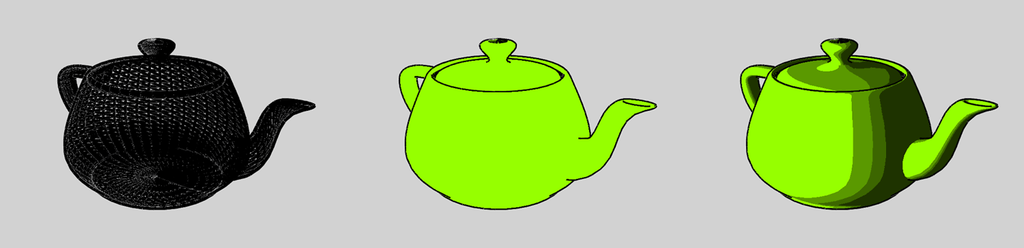
\includegraphics[width=\linewidth]{fig/teapots.png}
  \caption{Cel-shaded teapots. Image by Nicolas Sourd [CC-BY-SA-3.0 (http://creativecommons.org/licenses/by-sa/3.0/)], via Wikimedia Commons. (\url{https://goo.gl/5e6tNk}).}
\end{figure}

Duis sagittis massa odio, consequat ornare mauris imperdiet blandit. \cite{levoy:2000:TDM} Donec vel pulvinar nisl. Nam pretium vitae risus a consectetur. \cite{sako:2001:SSB, fedkiw:2001:VSO, Jobs95} Vestibulum efficitur auctor mauris. Vestibulum nec orci suscipit, faucibus mauris vel, elementum dolor. Phasellus ornare est id commodo cursus. Lorem ipsum dolor sit amet, consectetur adipiscing elit. Donec iaculis enim urna, vitae tincidunt est dictum id. Suspendisse lobortis justo id enim ornare euismod. Fusce quis turpis rhoncus, laoreet lorem eu, porttitor enim. \cite{kartch:2000:ERA, yee:2000:SSA, parke:1996:CFA} Etiam eget tempus velit. Duis iaculis id eros et mollis. Pellentesque non magna a massa rhoncus gravida id eget ex. Donec magna risus, posuere eu velit sit amet, tincidunt cursus leo. Curabitur non ultricies turpis, at sodales sapien.

\section{Related Works}
\label{sec:related}
Nullam mollis in lectus vitae tempus. Nam pellentesque tincidunt leo id dapibus. Etiam in euismod diam. \cite{ceres-solver, Asaro:1976:POT} Phasellus feugiat ante et dui rhoncus, at dictum elit vehicula. Nunc ut finibus neque. Sed vehicula tristique - as shown in Table \ref{soccer} - odio at interdum. Morbi ex lectus, porttitor vel ipsum id, scelerisque facilisis metus. Cras orci sapien, luctus in eros in, suscipit rhoncus neque. Duis pharetra elit vitae sagittis maximus. Curabitur fermentum justo massa, sed placerat odio aliquam quis. Nam facilisis hendrerit ante eget maximus. Nulla et porttitor nibh, et malesuada turpis. Suspendisse potenti. Nunc ultricies suscipit quam, eget ultrices nisi viverra vitae.

\begin{table}[ht]
\begin{center}
    \caption{Soccer, or football?}
\label{soccer}
\begin{tabular}{l*{6}{c}r}
Team              & P & W & D & L & F  & A & Pts \\
\hline
Manchester United & 6 & 4 & 0 & 2 & 10 & 5 & 12  \\
Celtic            & 6 & 3 & 0 & 3 &  8 & 9 &  9  \\
Benfica           & 6 & 2 & 1 & 3 &  7 & 8 &  7  \\
FC Copenhagen     & 6 & 2 & 1 & 3 &  5 & 8 &  7  \\
\end{tabular}
\end{center}
\end{table}

Aliquam sed vehicula neque. Praesent placerat, nisi sit amet condimentum porta, justo tellus dictum eros, quis vestibulum erat massa id sapien. Vestibulum euismod purus dolor, ornare consectetur quam egestas volutpat. Curabitur sollicitudin convallis purus ultrices facilisis. Pellentesque sollicitudin maximus orci quis rutrum. Phasellus a mauris maximus sem mollis sagittis. Vivamus sagittis faucibus tincidunt. Vivamus vel suscipit leo.

\begin{figure}[h]
  \centering
  \includegraphics[width=\linewidth]{fig/franklin}
  \caption{1907 Franklin Model D roadster. Photograph by Harris \& Ewing, Inc. [Public domain], via Wikimedia Commons. (\url{https://goo.gl/VLCRBB}).}
\end{figure}

\section{Proposal}
\label{sec:proposal}
Cum sociis natoque penatibus et magnis dis parturient montes, nascetur ridiculus mus. Vivamus maximus a lectus sed dictum. Curabitur pulvinar lectus nec magna molestie consequat. Donec ligula urna, scelerisque et felis sed, euismod feugiat sem. (See equation \ref{eqn:01}.) Donec urna libero, auctor sit amet sem id, malesuada tempor risus. Morbi malesuada lobortis consequat. Aliquam lacinia quam ac tristique sodales. Class aptent taciti sociosqu ad 
\begin{equation}
\label{eqn:01}
P(t)=\frac{b^{\frac{t+1}{T+1}}-b^{\frac{t}{T+1}}}{b-1},
\end{equation}
where $t=0,{\ldots}\,,T$, and $b$ is a number greater than $1$, litora torquent per conubia nostra, per inceptos himenaeos.

\begin{multline}
\label{the-rendering-equation}
L_o(x, \omega_o, \lambda, t) = L_e(x, \omega_o, \lambda, t)  + \\
\int_{\Omega} f_r(x, \omega_i, \omega_o, \lambda, t) L_i(x, \omega_i, \lambda, t)(\omega_i \cdot n) \text{d} \omega_i
\end{multline}

Lorem ipsum dolor sit amet, consectetur adipiscing elit. Fusce auctor accumsan nulla, vitae pharetra ipsum sagittis sit amet. Donec ac metus consectetur, venenatis magna sit amet, viverra sapien. Class aptent taciti sociosqu ad litora torquent per conubia nostra, per inceptos himenaeos. Phasellus eleifend sem sit amet arcu congue tempus. Proin at iaculis orci. (See equation \ref{the-rendering-equation}.) Pellentesque habitant morbi tristique senectus et netus et malesuada fames ac turpis egestas. Orci varius natoque penatibus et magnis dis parturient montes, nascetur ridiculus mus. Etiam feugiat dui sit amet ante pellentesque, sed malesuada libero ornare. Curabitur tempor ligula leo, in feugiat urna ornare luctus. Fusce quis metus sit amet neque sagittis elementum. Quisque facilisis quam quis tortor volutpat, et sodales urna efficitur.

\section{Implementation}
\label{sec:implementation}
The core idea of boids is put forward by Craig W. Reynolds in 1986~\cite{Reynolds:1987}. There is no need to implement a real commander which sends commands to each boid for maintaining the flock. Each individual only need to follow the 3 principles: alignment, cohesion, and separation.

To simulate the aggregate motion, for each boid, we iterate and collect both position and velocity(both speed and direction) information of all other flockmates to calculate average velocity, average distance to other flockmates, and central position of this flock. 

\subsection{Alignment}
The average velocity is used for alignment. The average velocity is a 3D vector with two parameters average heading and average speed. Each boid adjusts its heading towards the average heading of the whole flock so that the whole flock is always heading in the same direction. It also checks its speed with average speed. If the current boid is too fast, it slows down waiting for other flockmates catching up, otherwise speeds up. The more important part of the alignment is the heading match process. We notice that the speed alignment does not need to be specifically implemented since the separation process would be used to adjust speed instead. We set a minimum and a maximum speed for the flock and use Clamp function to adjust the speed. Heading is more important because it directly results in whether it’s jerky or smooth when the flock makes a turn. To achieve this, the following equation is implemented:
\vspace{3mm}
\begin{center}
$v_j = (\frac{1}{n}\sum_{i=1,i\neq{j}}^{n}{v_i})\cdot S + v_j \cdot (1-S)$
\end{center}
\vspace{3mm}
Where $v_j$ is the velocity of current boid, $n$ is the number of boids in the flock. $S$ is a parameter set to control the boid motion. Its value varies from 0 to 1. A larger $S$ means the changing vector takes more advantage than the current status so that the flock is more tending to change. The default setting of $S$ is 0.5. Thus, the changing vector is simplified to $v_{average} - v_j$. This change will attach to each boid by adding a force in the same direction as this changing vector. A weight value $w_a$ is set to determine the force strength. The final force add to the boid would be like this in our project implementation:
\vspace{3mm}
\begin{center}
$f_j = (v_{avg} - v_j)_{magnitude} \cdot w_a$
\end{center}
\vspace{3mm}
The whole process mentioned above is processed every frame to all boids.
\subsection{Cohesion}
Flock center position is used for cohesion. A force to the center of the flock is always added to each boid. Note that when flock crosses an obstacle, the boids may be divided into 2 or more parts then concentrate together again after then. In this case, there is no need to consider the center of each cluster when the flock is temporarily divided. Otherwise, the obstacle process of this may look like one flock initiated divide into two or more instead of an obstacle come across a single flock. The cohesion equation is:
\vspace{3mm}
\begin{center}
$v_j = ((\frac{1}{n}\sum_{i=1,i\neq{j}}^{n}{pos_i})-pos_j)\cdot S \cdot w_c + v_j \cdot (1-S)$
\end{center}
\vspace{3mm}
Here $pos$ is the position of a boid, $w_c$ is the weight of cohesion. We could see that the further boid[j] away from the center of the flock, a larger force will be implemented.

\subsection{Separation}
Average boid distance is used for separation. We set a collision test for each boid in the flock to make them separate. Each boid has a private zone and we check whether other flockmates entered this zone. If so, a separation force is added each frame until leaving. The equation is like the following:
\vspace{3mm}
\begin{center}
$v_j = (\frac{1}{n}\sum_{i=1,i\neq{j}}^{n}{\frac{v_i}{dist(pos_i,pos_j)}})\cdot S \cdot w_s + v_j \cdot (1-S)$
\end{center}
\vspace{3mm}
$dist(pos_i,pos_j)$ is distance vector from boid[i] to boid[j]. The further boid[i] away from boid[j] the less influence will be added for separation. The private zone mentioned above is set to avoid unnecessary calculation. We consider both the position and velocity of other flockmates in this process. We notice that if only the position of two boids is considered, the flock could not be separated well in some situations (e.g. When boids are too close to each other at the beginning). This is also used for the speed matching process that we mentioned in the alignment section. A separation weight parameter $w_s$ is also set for separation force.\break
%\vspace{5mm}
\\
The $S$ parameter from 3 equations have the same function and set to be the same in our implementation but it does not necessary to be the same. The 3 weight value are all set to be 1, it is does not make a significant change to the output when the value changes. We believe they are not necessary parameters. Recall the algorithm mentioned in this section is only implemented to each boid and no other general control system is added. This is built to stick to the natural flock condition.

\section{Optimization}
\label{sec:optimization}
Based on the 3 rules we further implement two other optimization approaches of our own. 

First, iterating all flockmates for each boid per frame is too expensive and may cause tones of lagging or even crashing. We took Sebastian Lague’s project as reference and implemented a GPU based multi-thread iteration for calculating the 3 key parameters mentioned above. This time each boid has one thread on gpu and iterates simultaneously. 

We also add a random force to each boid every 20 frames. In some situation(e.g. When the flock move straight forward for a time), the boids situation keeps no change and make the whole flock look too ordered and becomes even sterile. So an uneven force with random direction is added to make more change to the flock motion. This force is not designed to completely break the flock order and reform again. It’s order to downgrade the precision of computer calculation and make the motion more realistic.

\subsection{Avoid Obstacle}

The interaction with obstacle object is the most interesting part of the whole simulation. It makes the flock motion more random and unpredictable when it comes across an object with complex shape. Sometimes the boids could be divided into several smaller groups but the whole motion looks still smooth and you could feel that the small clusters still forming one single flock. 

The strategy to achieve this is complicated. Craig W. Reynolds mentioned two different attempts: force field model and steer-to-avoid, and we implemented the latter one. We designed several rays sending from the front of the boids to detect if there are obstacles ahead. But directly detecting the collision of rays on the surface of object could be very expensive if the object is polehydural. We simplify this question by casting the obstacle into a sphere. In this case for each ray sent from boid, the obstacle could be casted into a circle on a 2D panel with this ray. With this cast we solve 2 problems together, the complexity of directions in 3D and arbitrary shape of obstacles. 

When an obstacle is detected, a normalized force will be added to the boid on the same panel of the detection ray. This force is designed to turn the heading of the current boid and the angle it turns will be based on golden ratio. In some simplified cases, for example if a boid heading perpendicular to a flat surface, the boid will steer a golden spiral to avoid collision. This is designed to avoid shape turns and make the whole process smooth and natural. Since the flock is still maintaining during the avoid process, the avoid force is added on the 3 rules and it is not necessary to worry the force from the 3 rules may affect the performance of avoiding.


\subsection{Prey and Predator}

To test the durability of our system, we introduced a prey and predator into our system to simulate a real natural scene.

The prey randomly pick a point in the scene and move toward that point. To make the motion of prey smooth and real, we implement a force from the position of prey to the target point on prey each frame. When the prey reaches the target, another point will be randomly picked. The flock chases the prey by a similar way. A force heading the prey is added on boid each frame together with 3 rules. 

We also added a predator to chase the flock. The predator is always heading the center of flock and the strategy is exactly the same as boid chasing prey. Each boid get an updated predator position each frame. If the distance of predator is less than an avoid radius an escape force will be added toward an opposite direction of predator on boid. The difference between avoid predator and obstacles is the boids do not follow 3 rules when escaping predators. We notice that 3 rules should not be implemented to simulate this process like what it usually happen in nature.


\section{Conclusions}
\label{sec:conclusions}
Nullam vulputate enim ut tortor mollis pharetra. Cras pellentesque sem a accumsan malesuada. Donec at massa nisl. Sed malesuada felis id nisl maximus efficitur. In pretium metus non faucibus pulvinar. Sed pulvinar elit ultrices mauris vehicula, id ultricies purus finibus. Fusce tempus elit molestie, consequat ipsum eget, iaculis nibh. Cras tincidunt, orci in lacinia tempus, mauris leo finibus orci, vitae dignissim dui risus et odio. Sed commodo ultricies nulla, et varius velit aliquam quis. Sed efficitur, ex non facilisis dignissim, lacus orci accumsan massa, dictum facilisis arcu lacus ac leo. Sed quis tellus dictum massa egestas dapibus vel et justo. Nulla euismod lectus ut purus hendrerit porttitor. Suspendisse quis dui ligula. Proin non porta libero. Maecenas vel feugiat urna.

\bibliographystyle{ACM-Reference-Format}
\bibliography{main}
\end{document}